\subsection{Vergleich der Informationsquellen}\label{subsec:vergleich}
Im Zuge des Vergleich wurden 30 Vendors (n=30) nach Vorhandensein der Informationsquellen ausgewertet. Als Informationsquellen wurden RSS-Feeds, Twitter und Newsletter ausgew�hlt. Ein weiteres Kriterium in der Auswertung ist das Datum des letzten Updates. Das Datum wird nach dem neuesten Eintrag zwischen den vorliegenden Informationsquellen zum Zeitpunkt 10.05.2017 bestimmt. Die Zusammenfassung der Ergebnisse wird in Tabelle \ref{tab:vergleich} dargestellt: 
\begin{table}[H] 
\centering 
\begin{tabular}{ |l|c|c|c|c| }
\hline
\textbf{Vendor} & \textbf{RSS} & \textbf{Twitter} & \textbf{Newsletter} & \textbf{Last Update} \\ \hline
\hline
Anynines & nein & ja & ja & 18.08.15 \\ \hline
App42 PaaS & nein & ja & nein & 10.05.17 \\ \hline
AppFog & nein & ja & ja & 10.05.17 \\ \hline
AppHarbor & nein & ja & nein & 22.05.16 \\ \hline
BitNami & nein & ja & nein & 10.05.17 \\ \hline
Brightbox & nein & ja & nein & 25.04.17 \\ \hline
Clever Cloud & nein & ja & nein & 26.04.17 \\ \hline
Cloudnode & nein & ja & nein & 23.04.17 \\ \hline
CloudUnit & nein & ja & nein & 10.05.17 \\ \hline
Cloudways & nein & ja & ja & 10.05.17 \\ \hline
EngineYard & nein & ja & nein & 29.04.17 \\ \hline
Flynn & nein & ja & ja & 17.10.16 \\ \hline 
fortrabbit & nein & ja & nein & 04.05.17 \\ \hline
Getup Cloud & nein & ja & nein & 09.05.17 \\ \hline
Google App Engine & nein & ja & ja & 10.05.17 \\ \hline
Heroku & ja & ja & ja & 10.05.17 \\ \hline
Jelastic & nein & ja & ja & 10.05.17 \\ \hline
Mendix & nein & ja & nein & 28.04.17 \\ \hline
mOSAIC & ja & nein & nein & 05.04.13 \\ \hline
OpenShift Container Platform & nein & ja & nein & 22.04.17 \\ \hline
Oracle Cloud PaaS & ja & ja & nein & 01.12.16 \\ \hline
OrangeScape & nein & ja & nein & 05.04.17 \\ \hline
Pagoda Box & nein & ja & nein & 06.05.16 \\ \hline
Platformer.com & ja & ja & nein & 01.04.17 \\ \hline
SAP HANA Cloud Platform & nein & ja & nein & 02.05.17 \\ \hline
Software AG Live & nein & ja & nein & 10.05.17 \\ \hline
Tsuru & nein & ja & ja & 12.04.17 \\ \hline
Voxoz & nein & ja & nein & 08.01.17 \\ \hline
WSO2 App Cloud & nein & ja & ja & 10.05.17 \\ \hline   
\end{tabular}
\caption {Vergleich der Informationsquellen (RSS, Twitter und Newsletter)} 
\label{tab:vergleich}
\end{table} 
In Bezug auf Web-Feeds spricht man von \glqq{}Content Syndication\grqq{}, was im deutschsprachigen Raum als \glqq{}Syndikation\grqq{} bezeichnet wird. Unter Syndikation wird Bereitstellung von Daten f�r �bertragung, Aggregierung und Online-Publikation\footnote{http://web.resource.org/rss/1.0/} verstanden. Ein verbreitetes Format f�r Web-Feeds ist RSS. Urspr�nglich fand RSS besondere Verbreitung bei Webbloggern \cite[S.103]{tilkov2015}. Aufgrund des einfachen Konzeptes ist RSS in k�rzer Zeit zum meistgenutzten Format zur �nderungsbenachrichtigung geworden.\\
Je nach Quelle wird die Abk�rzung RSS unterschiedlich interpretiert. In der ersten Version (RSS 1.0) stand die Abk�rzung f�r \glqq{}RDF Site Summary\grqq{}. In der Version 2.0 wird jedoch \glqq{}Really Simple Syndikation\grqq{}\footnote{https://validator.w3.org/feed/docs/rss2.html\label{rss2.0}} erw�hnt. Ein RSS 2.0 Dokument wird in XML-Format definiert und als Wurzel den Rss-Tag enth�lt, der den Namensraum der Elemente und die Version von RSS bestimmt. Im Rss-Tag wird der Channel-Tag definiert, der folgende Elemente enthalten muss (siehe \ref{rss2.0}):
\begin{itemize}
\item Title: Name des Channels (engl. Kanal)
\item Link: URL zur Webseite des entsprechenden Channels
\item Description: kurze Zusammenfassung des Channels
\end{itemize} 
Die Inhalte des Channels werden durch Items dargestellt. Laut der Spezifikation in \ref{rss2.0} entspricht ein Item einer Story (ein kurzer Artikel). Bei einem Item gibt es keine Pflichtfelder. Allerdings muss entweder Title oder Description vorhanden sein. Ein Beispiel f�r einen RSS 2.0 Feed\footnote{https://blog.heroku.com/news/feed} wird in Listing \ref{rss} dargestellt.
\begin{lstlisting}[basicstyle=\ttfamily, breaklines=true, label=rss,
					captionpos=b, caption={Beispiel eines Eintrages in RSS 2.0}]
<rss xmlns:dc="http://purl.org/dc/elements/1.1/" version="2.0">
 <channel>
  <title>Heroku</title>
  <link>http://blog.heroku.com</link>
  <description>The Heroku Blog</description>
  <item>
   <title>The Heroku-16 Stack is Now Available</title>
   <link>https://blog.heroku.com/heroku-16-is-generally-available</link>
   <pubDate>Thu, 20 Apr 2017 15:06:00 GMT</pubDate>
   <guid>https://blog.heroku.com/heroku-16-is-generally-available</guid>
   <description>
    <p>Your Heroku applications run on top of ...</p> 
   </description>
   <author>Jon Byrum</author>
  </item>
 </channel>
</rss>
\end{lstlisting}
Im Beispiel von Heroku werden au�erdem separate Feed-Channels f�r die unterschiedlichen Themenbereiche angeboten, wie es in Abbildung \ref{fig:heroku-feeds} zu sehen ist.
\begin{figure}[H] 
	\centering
	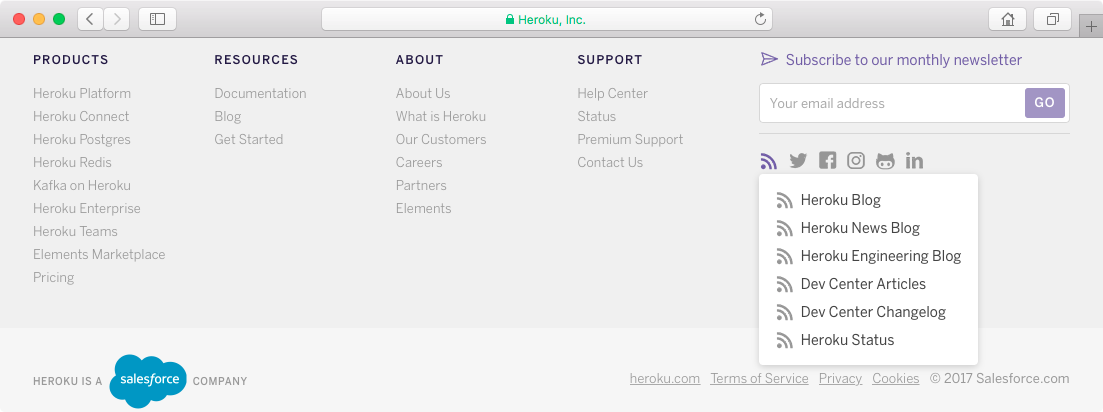
\includegraphics[width=1.0\textwidth]{images/heroku-feeds.png}
	\caption{Feed-Channels von Heroku}
	\label{fig:heroku-feeds}
\end{figure}
Der Themenbereich umfasst sowohl allgemeine (z.B. Heroku Blog) als auch spezifische Informationen (z.B. Dev Center Articles). Im Anwendungsfall von \textit{PaaSfinder} ist der Dev Center Changelog Channel besonders relevant, da der die Benachrichtigungen im technischen Bereich enth�lt (siehe Abbildung \ref{fig:heroku-changelog-feed}).
\begin{figure}[H] 
	\centering
	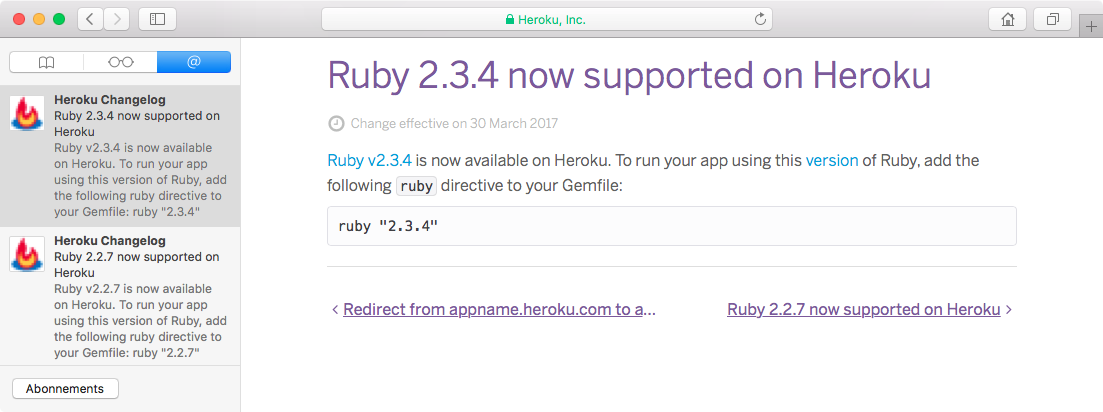
\includegraphics[width=1.0\textwidth]{images/heroku-changelog.png}
	\caption{Heroku Feed}
	\label{fig:heroku-changelog-feed}
\end{figure}
Neben RSS k�nnen die Daten aus sozialen Netzwerken erschlossen werden. Zu diesem Zweck stellen die Anbieter der sozialen Netzwerken (z.B. Facebook\footnote{https://developers.facebook.com/docs/graph-api/}, Twitter\footnote{https://dev.twitter.com/overview/api}) eine REST-API zur Verf�gung, die das Lesen/Schreiben der Daten erm�glicht. Im Beispiel von Heroku hat sich herausgestellt, dass sich Twitter am besten f�r Benachrichtigungen geeignet ist. Bei diesem konkreten Fall handelt es sich sogar um die gleiche Information wie in RSS-Feeds (vgl. Heroku in Abbildung \ref{fig:heroku-changelog-feed} und \ref{fig:heroku-twitter}).
\begin{figure}[H] 
	\centering
	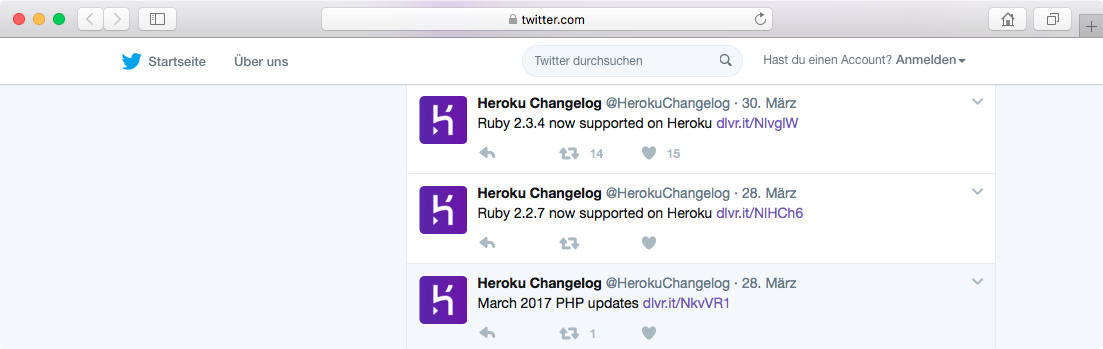
\includegraphics[width=1.0\textwidth]{images/twitter.png}
	\caption{Heroku Twitter}
	\label{fig:heroku-twitter}
\end{figure}
Es bleibt also dem Entwickler offen, ob man sich f�r einen News-Dienst wie Twitter oder Web-Feeds entscheidet. In beiden F�llen kommt man auf die gleiche Information, die unterschiedlich repr�sentiert wird. W�hrend Twitter eine umfangreiche REST-API mit Daten in JSON Format anbietet, setzt RSS auf das XML-Format. Die RSS-Daten k�nnen mit dem HTTP-GET-Request aufgerufen werden.\\
Unabh�ngig davon, ob die Datenerfassung �ber Twitter API oder RSS erfolgt, k�nnen die Daten wiederum an die Worker-API gesendet werden. Im einfachsten Fall werden sie an das Github-Repository weitergegeben. In der fortgeschrittenen Variante k�nnen die Daten nach bestimmten Kriterien gefiltert bzw. verarbeitet werden. 